\documentclass[pdftex,12pt,a4paper]{report}

\usepackage[pdftex]{graphicx}
\usepackage{float}
\usepackage{fancyvrb}
\fvset{xleftmargin=2em}
\usepackage{multicol}
\usepackage{wrapfig}

\usepackage{pgfplots}
\pgfplotsset{width=10cm,compat=1.9}
\usepackage{tikzscale}
\usepackage{pgfplotstable}
\usepackage{booktabs}
\usepackage[font=small,labelfont=bf,tableposition=top]{caption}

\usepackage[utf8]{inputenc} % isto é um comentário
\usepackage[portuges]{babel}
\usepackage[T1]{fontenc}
\usepackage{times}
%\usepackage{lmodern}
\usepackage[obeyspaces,spaces]{url}
\usepackage[left=25mm,right=25mm,top=25mm,bottom=25mm]{geometry}
\usepackage{titlesec}
\usepackage{mathtools}
%identa 1º paragrafo de capitulos e secções
\usepackage{indentfirst}

\newcommand{\HRule}{\rule{\linewidth}{0.5mm}}
\titleformat{\chapter}{\normalfont\huge}{\thechapter.}{20pt}{\huge}


\begin{document}

\begin{titlepage}


\begin{minipage}{0.3\textwidth}
\begin{flushleft} 

\includegraphics[width=\textwidth]{logo.png}
\end{flushleft}
\end{minipage}
\begin{minipage}{0.6\textwidth}
\begin{flushright} 

\textsc{Departamento de Engenharia Informática}\\[0.1cm]
\bfseries Mestrado Integrado em Engenharia Informática \\ [0.1cm]
\bfseries \textit{Sistemas Operativos}\\[8mm]

\end{flushright}
\end{minipage}


\vspace{3cm}


\begin{center}



\Large \textbf{\textit{Processamento de NoteBooks}}\\[1.5cm]


{\Large \bfseries Grupo 46\\[2cm] }


\noindent\begin{minipage}[b]{.1\textwidth}
	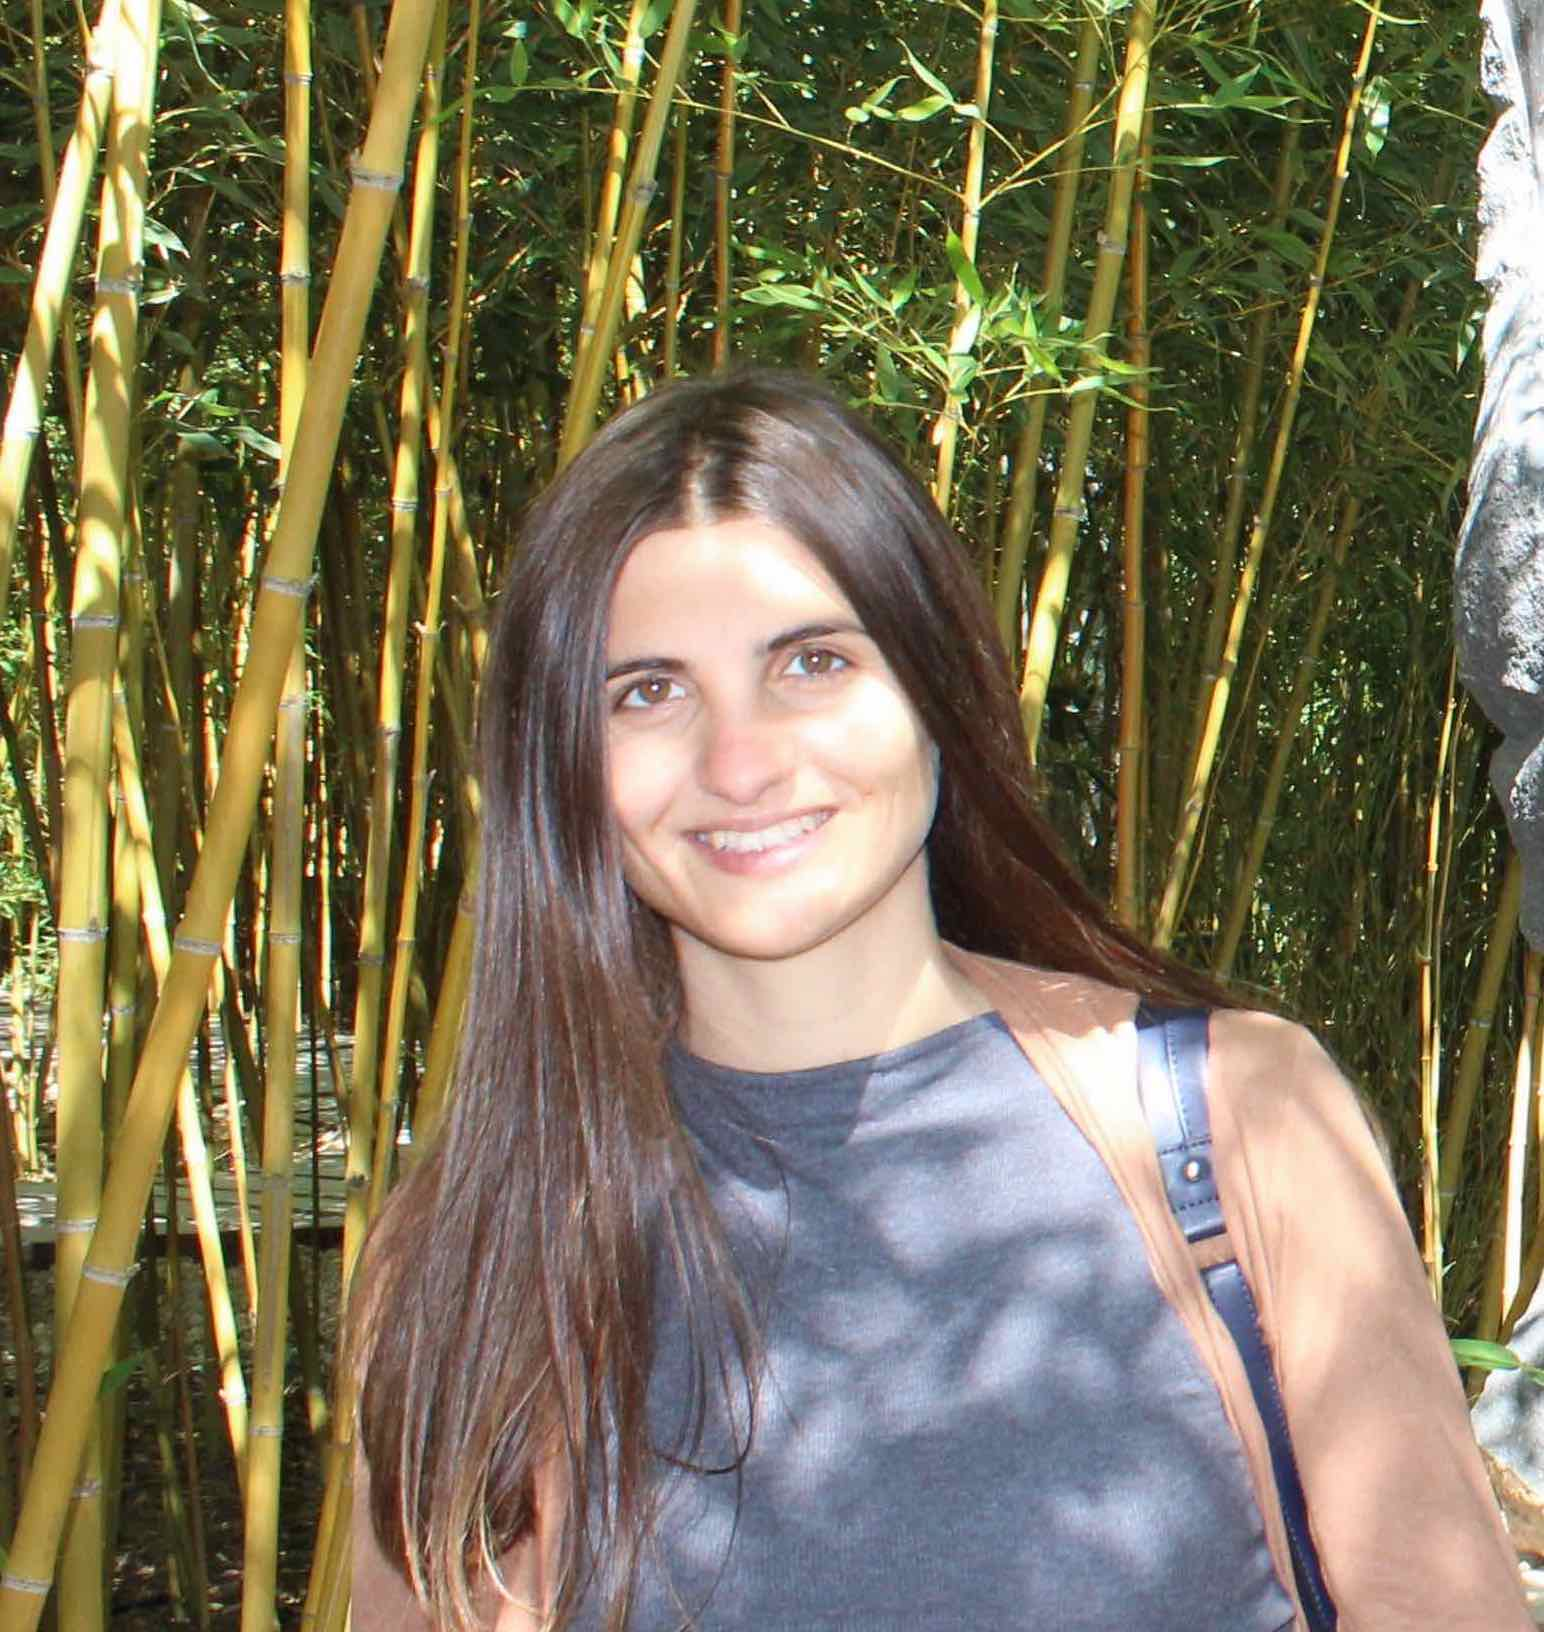
\includegraphics[scale=0.1]{celia}
	\small{Célia Figueiredo ae3698}
\end{minipage} 
\hfill
\begin{minipage}[b]{.1\textwidth}
	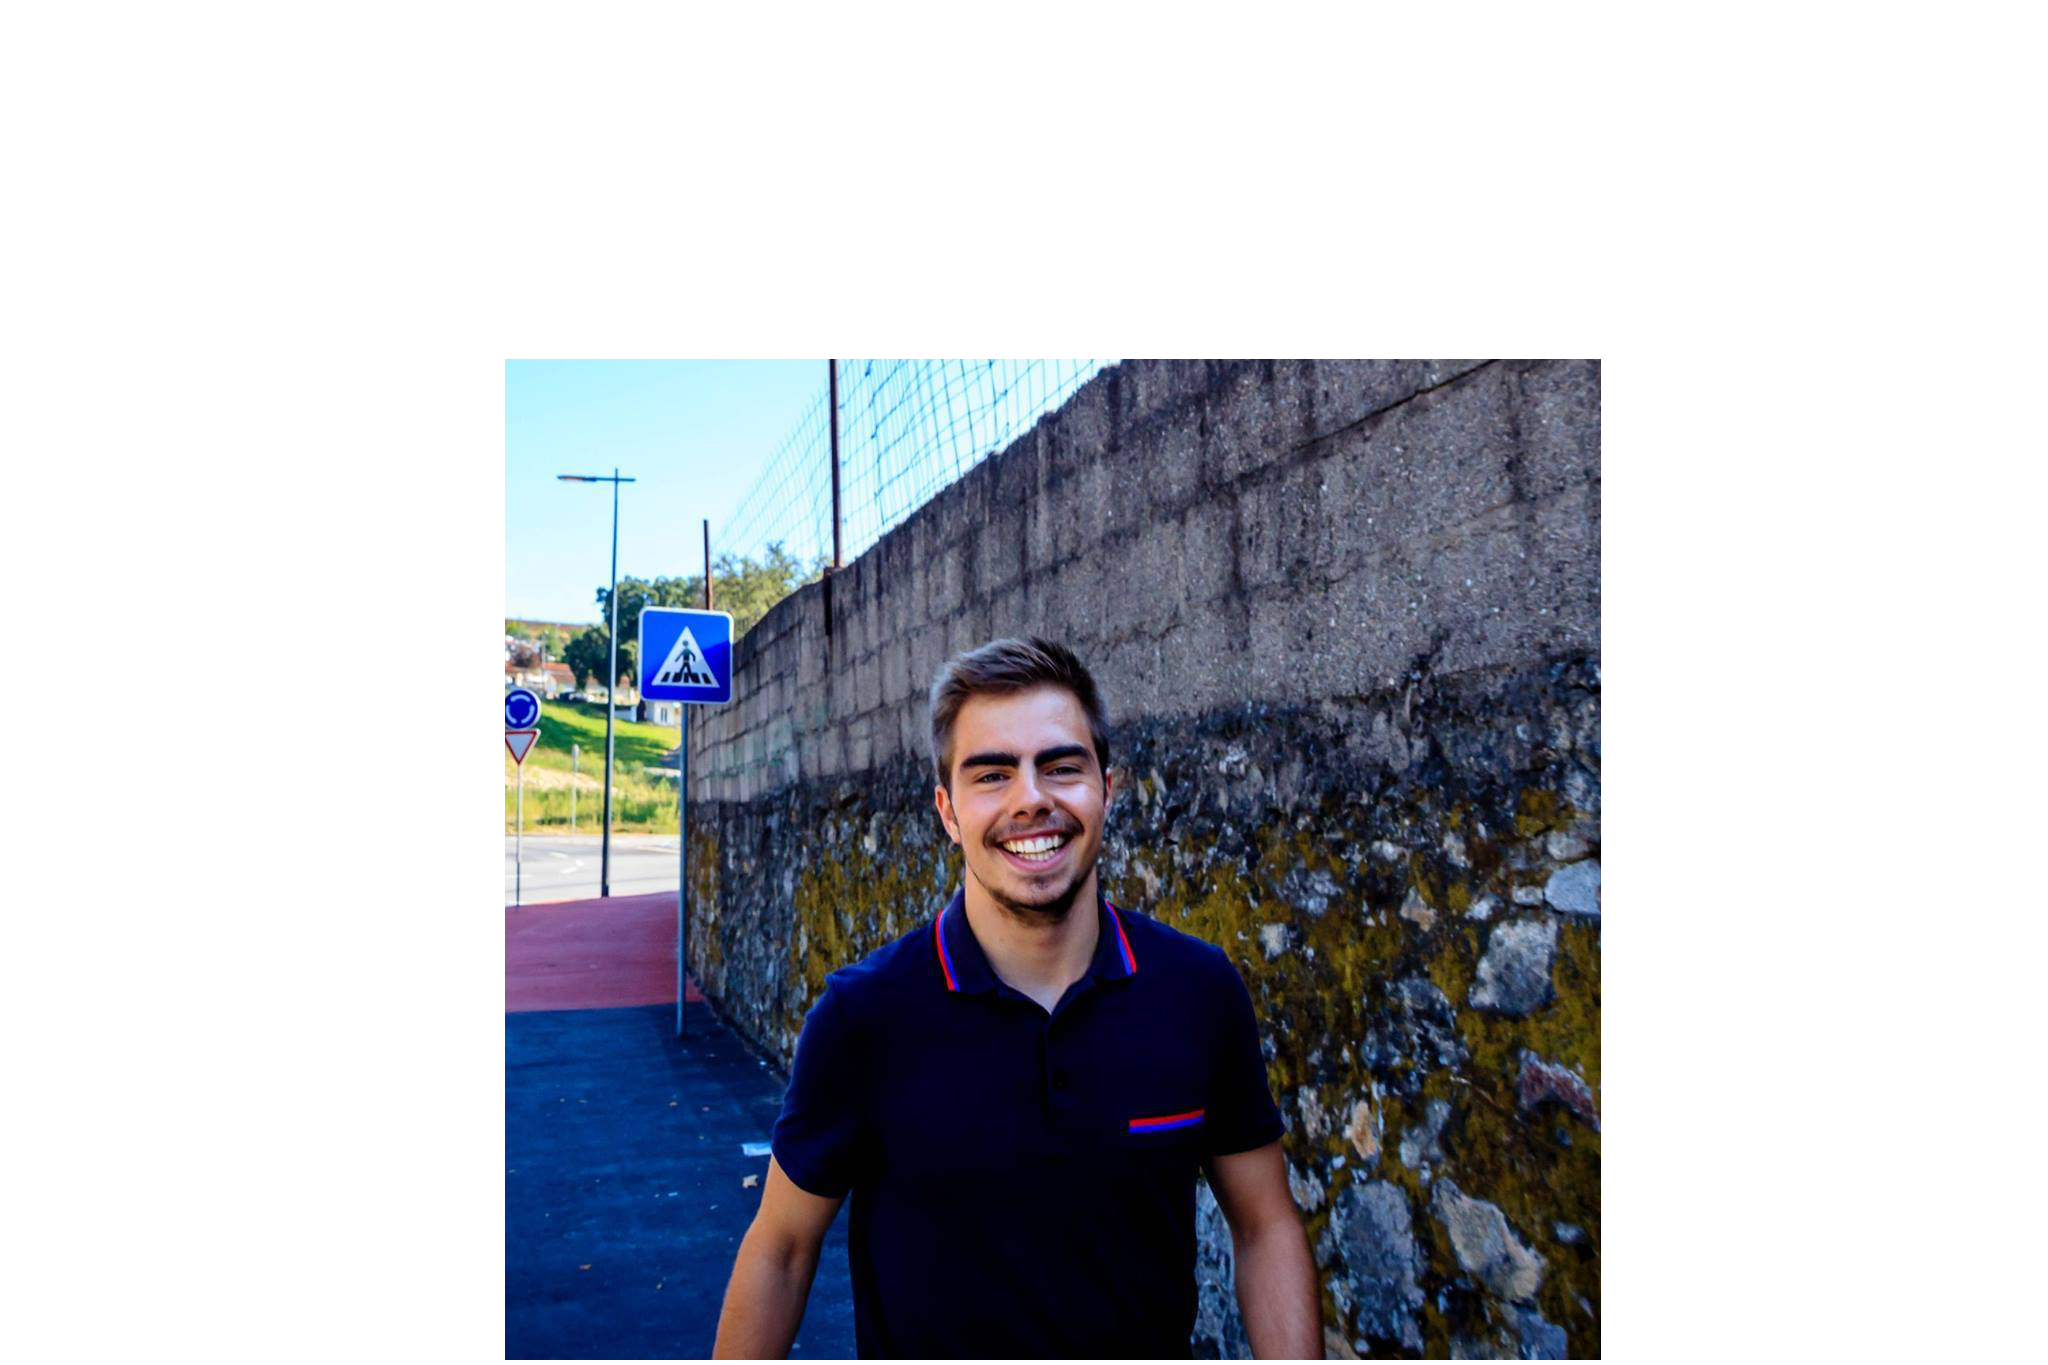
\includegraphics[scale=0.1]{squirtle}
	\small{Ricardo Pereira a7}
\end{minipage}
\hfill
\begin{minipage}[b]{.2\textwidth}
	
\includegraphics[scale=0.2001]{marcia}
	\small{Márcia Costa a67672}
\end{minipage}




\vspace{3ex}


\vfill

\large Braga, {\large \today}

\end{center}
\end{titlepage}


\tableofcontents

\begin{abstract}

O documento descreve o trabalho efetuado para a realização do projeto, onde foi pedida a implementação de um sistema para processamento de \textit{notebooks}, que misturam fragmentos de código, resultados da execução e documentação. Um \textit{notebook} é um ficheiro de texto que depois de processado é modificado de modo a incorporar resultados de exceção de código ou comandos nele embebidos. 

\end{abstract}
\chapter{Introdução}
\label{cap:intro}

O presente relatório documenta o trabalho prático referente a Unidade Curricular de Sistemas Operativos pertencente ao plano de estudos do 2º ano do Mestrado Integrado em Engenharia Informática.



\chapter{Descrição geral do projeto}
\section{Notebook}


\chapter{Arquitetura das Classes}

\chapter{Funcionamento da Aplicação UMeR}
\section{Menu Inicial}
\chapter{Conclusões }

Com a realização deste trabalho pode-se concluir que ainda há aspetos a melhorar, tais como a apresentação dos menus, poder-se-ia ter melhorado a organização, por exemplo as estatisticas que são acedidas pelo administrador deviam ter um menu de introdução de estatisticas. 



\section{Trabalho Futuro}

Como trabalho futuro a aplicação poderá vir a permitir registo de empresas e a utilização das filas de espera dos veiculos, para o primeiro ponto ter-se-ia de adicionar um novo tipo de utilizador e dar-lhe permissão para conseguir gerir os seus motoristas e veiculos.  Para o segundo seria necessário alterar a requisição de um veiculo e  se ele permitisse fila de espera adicionar o cliente a essa fila e alterar o estado do cliente para em fila de espera, caso o veiculo estivesse ocupado. 





\end {document}


